\documentclass[border=5pt]{standalone}
\usepackage{fontspec}
\usepackage{unicode-math}
\setmainfont{Noto Serif}
\newfontfamily\FigureItalic{Noto Serif}
\setmathfont{STIXTwoMath-Regular.otf}
\usepackage{tikz}
\usetikzlibrary{arrows.meta,calc,patterns,decorations.pathmorphing,decorations.markings,decorations.pathreplacing,positioning,backgrounds}
\definecolor{Ink}{HTML}{000000}
\definecolor{Curve}{HTML}{000000}
\definecolor{Bzero}{HTML}{000000}
\definecolor{Bone}{HTML}{000000}
\definecolor{Btwo}{HTML}{000000}
\definecolor{Bthree}{HTML}{000000}
\definecolor{Bfour}{HTML}{000000}
\tikzset{
 ax/.style={draw=Ink,line width=.72pt,-{Latex[length=2.4mm,width=1.5mm]}},
 lev/.style={draw=Ink,line width=1.4pt,line cap=butt},
 thinlev/.style={draw=Ink,line width=.65pt,line cap=butt},
 helper/.style={draw=Ink,line width=.65pt},
 bare/.style={draw=Ink,line width=.95pt,dash pattern=on 4pt off 2.8pt},
 curve/.style={draw=Ink,line width=1.85pt,line cap=round,line join=round},
 ray/.style={draw=Ink,line width=1.0pt,-{Latex[length=2.3mm,width=1.4mm]}},
 measure/.style={draw=Ink,line width=.75pt,{Latex[length=1.9mm,width=1.2mm]}-{Latex[length=1.9mm,width=1.2mm]}},
 link/.style={draw=Ink,line width=1.0pt},
 wave/.style={draw=Ink,line width=.85pt,decorate,decoration={snake,amplitude=.33mm,segment length=2.5mm,pre length=.8mm,post length=.8mm}},
 photon/.style={draw=Ink,line width=1.0pt,-{Latex[length=2.0mm,width=1.3mm]},decorate,decoration={snake,amplitude=.4mm,segment length=2.7mm,pre length=0mm,post length=1.9mm}},
 lab/.style={text=Ink,font=\fontsize{13.5}{16}\selectfont,inner sep=2pt},
 small/.style={text=Ink,font=\fontsize{11.5}{14}\selectfont,inner sep=2pt},
 tag/.style={text=Ink,font=\fontsize{14}{17}\selectfont\FigureItalic\itshape,inner sep=2pt}}
\pagestyle{empty}

\begin{document}
% FIG-10.1: source-checked reconstruction V2, 2026-11-04.
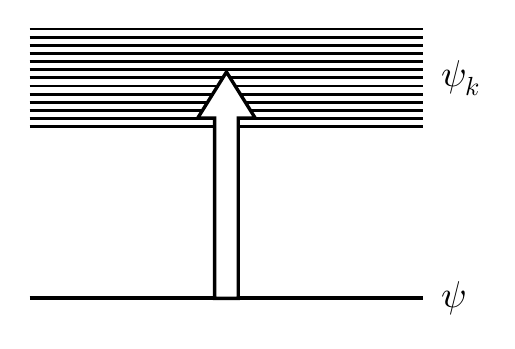
\begin{tikzpicture}[x=1cm,y=1cm]
% Figure 10.1, p.121; equations (10.1)-(10.4).
% Upper states are one zone; no intrazone transition arrows are implied.
\draw[lev] (1.000000,0.400000)--(6.000000,0.400000);
\node[lab,anchor=west] at (6.150000,0.400000) {$\psi$};
\draw[link] (1.000000,2.580000)--(6.000000,2.580000);
\draw[link] (1.000000,2.683333)--(6.000000,2.683333);
\draw[link] (1.000000,2.786667)--(6.000000,2.786667);
\draw[link] (1.000000,2.890000)--(6.000000,2.890000);
\draw[link] (1.000000,2.993333)--(6.000000,2.993333);
\draw[link] (1.000000,3.096667)--(6.000000,3.096667);
\draw[link] (1.000000,3.200000)--(6.000000,3.200000);
\draw[link] (1.000000,3.303333)--(6.000000,3.303333);
\draw[link] (1.000000,3.406667)--(6.000000,3.406667);
\draw[link] (1.000000,3.510000)--(6.000000,3.510000);
\draw[link] (1.000000,3.613333)--(6.000000,3.613333);
\draw[link] (1.000000,3.716667)--(6.000000,3.716667);
\draw[link] (1.000000,3.820000)--(6.000000,3.820000);
\node[lab,anchor=west] at (6.150000,3.200000) {$\psi_k$};
\path[draw=black,fill=white,line width=1.22pt,line join=miter]
 (3.350,0.400) -- (3.650,0.400) -- (3.650,2.690) -- (3.865,2.690)
 -- (3.500,3.275) -- (3.135,2.690) -- (3.350,2.690) -- cycle;
\end{tikzpicture}

\end{document}
